\section{Auswertung und Diskussion}
\label{sec:Auswertung und Diskussion}
\subsection{Bestimmung der Gegenspannung $U_g$}
Zur Bestimmung der Gegenspannung  wird  für verschiedene Wellenlänge des eingestrahlten Lichtes der
Elektronenstrom I in Abhängigkeit von der Spannung U der Photozelle gemessen.
Wegen der parabolischen Zusammenhang wird die Wurzel des gemessenen Photostroms
gegen die jeweilige angelegte Spannung aufgetragen.
Die Ausgleichungsgerade hat die Form
\begin{equation}
  \sqrt{I}= a\cdot U+b.\\
\end{equation}
Der Schnittpunkt dieser linearen Ausgleichsgeraden mit der U-Achse (bei $I=0\, \text{A}$) stellt nun den gesuchten Wert
für $U_g$ dar. Er berechnet sich nach
\begin{equation}
U_g= \frac{-b}{a}.\\
\end{equation}
Der Fehler für die Gegenspannung $U_g$  wird dabei über die Gau"s´sche Fehlerfortfplanzung 
  \begin{equation}
    \nonumber
      \Delta f = \sqrt{\sum_{i=1}^N {\Bigl(\frac{\partial f}{\partial y_i}\Bigr)^2 (\Delta y_i)^2}}\\
  \end{equation}
  \begin{align*}
   \Delta U_g =\sqrt{\Bigl(- \frac{1}{a} \cdot \Delta b \Bigr)^2+\Bigl(-b\cdot \frac{-1}{a^2} \cdot \Delta a\Bigr)^2}\\
  \end{align*}
  berechnet.

  \begin{table}[H]
    \centering
    \caption{Die Messdaten von rotes Licht $\lambda = 640 \,\text{nm}$ }
    \label{tab:rot}
    \begin{tabular}{| c | c |c||c|c|c| }
    \toprule
    $U/\mathrm{V}$ &$I/\mathrm{nA}$  &  $\sqrt{I}/\sqrt{\mathrm{nA}}$&$U/\mathrm{V}$ & $I/\mathrm{A} $& $\sqrt{I}/\sqrt{\mathrm{nA}}$  \\
    \midrule
    -0,23	& 0,000	& 0,000	& 0,40	& 0,036	 & 0,190\\
    -0,20	& 0,000	& 0,000	& 0,45	& 0,040	 & 0,200\\
    -0,15	& 0,001	& 0,032	& 0,50	& 0,043	 & 0,207\\
    -0,10	& 0,002	& 0,045	& 0,55	& 0,046	 & 0,214\\
    -0,05	& 0,003	& 0,055	& 0,60	& 0,048	 & 0,219\\
    0,00	& 0,005	& 0,071	& 0,65	& 0,050	 & 0,224\\
    0,05	& 0,008	& 0,089	& 0,70	& 0,053	 & 0,230\\
    0,10	& 0,012	& 0,110	& 0,75	& 0,055	 & 0,235\\
    0,15	& 0,016	& 0,126	& 0,80	& 0,057	 & 0,239\\
    0,20	& 0,020	& 0,141	& 0,85	& 0,058	 & 0,241\\
    0,25	& 0,024	& 0,155	& 0,90	& 0,060	 & 0,245\\
    0,30	& 0,028	& 0,167	& 0,95	& 0,062	 & 0,249\\
    0,35	& 0,032	& 0,179	& 1,00	& 0,064	 & 0,253\\
    \bottomrule
    \end{tabular}
  \end{table}
  \noindent
  \begin{figure}[H]
    \centering
    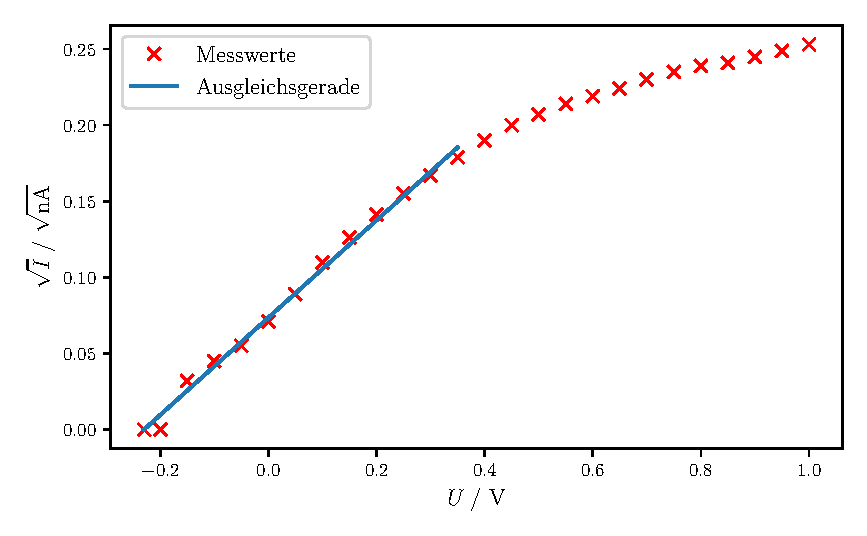
\includegraphics{rot.pdf}
    \caption{Grafik zur Bestimmung der Gegenspannung für rotes Licht $ \lambda = 640\, \text{nm}$.}
    \label{fig:rot}
  \end{figure}
  \noindent
  \begin{table}[H]
    \centering
    \caption{Die Messdaten von gelbes Licht $\lambda = 579,1 \,\text{nm}$ }
    \label{tab:gelb}
    \begin{tabular}{| c | c |c||c|c|c| }
    \toprule
    $U/\mathrm{V}$ &$I/\mathrm{nA}$  &  $\sqrt{I}/\sqrt{\mathrm{nA}}$&$U/\mathrm{V}$ & $I/\mathrm{A} $& $\sqrt{I}/\sqrt{\mathrm{nA}}$  \\
    \midrule 
    -19,14	& -0,020	&	        &  0,3	   &   0,056	& 0,237   \\
    -12,00	& -0,020	&	        &  0,4	   &   0,072	& 0,268   \\
    -10,00	& -0,020	&	        &  0,5	   &   0,086	& 0,293   \\
    -8,00	  & -0,020	&	        &  0,6	   &   0,100	& 0,316   \\
    -6,00	  & -0,020	&	        &  0,7	   &   0,110	& 0,332   \\
    -4,00	  & -0,020	&	        &  0,8	   &   0,125	& 0,354   \\
    -3,00	  & -0,020	&	        &  0,9	   &   0,135	& 0,367   \\
    -2,00	  & -0,020	&	        &  1	     &   0,150	& 0,387   \\
    -1,00	  & 0,000	  & 0,000	  &  1,1	   &   0,160	& 0,400   \\
    -0,90	  & 0,000	  & 0,000	  &  2	     &   0,220	& 0,469   \\
    -0,80	  & 0,000	  & 0,000	  &  3	     &   0,275	& 0,524   \\
    -0,70	  & 0,000	  & 0,000	  &  4	     &   0,320	& 0,566   \\
    -0,66	  & 0,000	  & 0,000	  &  5	     &   0,340	& 0,583   \\
    -0,5	  & 0    	  & 0,000	  &  7	     &   0,4	  & 0,632   \\
    -0,4	  & 0,002	  & 0,045	  &  9	     &   0,42	  & 0,648   \\
    -0,3	  & 0,002	  & 0,045	  &  11	     &   0,44	  & 0,663   \\
    -0,2	  & 0,004	  & 0,063	  &  15	     &   0,48	  & 0,693   \\
    -0,1	  & 0,012	  & 0,110	  &  17	     &   0,48	  & 0,693   \\
    0,02	  & 0,02	  & 0,141	  &  17,5    &   0,5	  & 0,707   \\
    0,1	    & 0,03	  & 0,173	  &  19	     &   0,5	  & 0,707   \\
    0,2	    & 0,042	  & 0,205	  &  		     &          &         \\ 
    
    
    \bottomrule
    \end{tabular}
  \end{table}
  \noindent

  \begin{figure}[H]
    \centering
    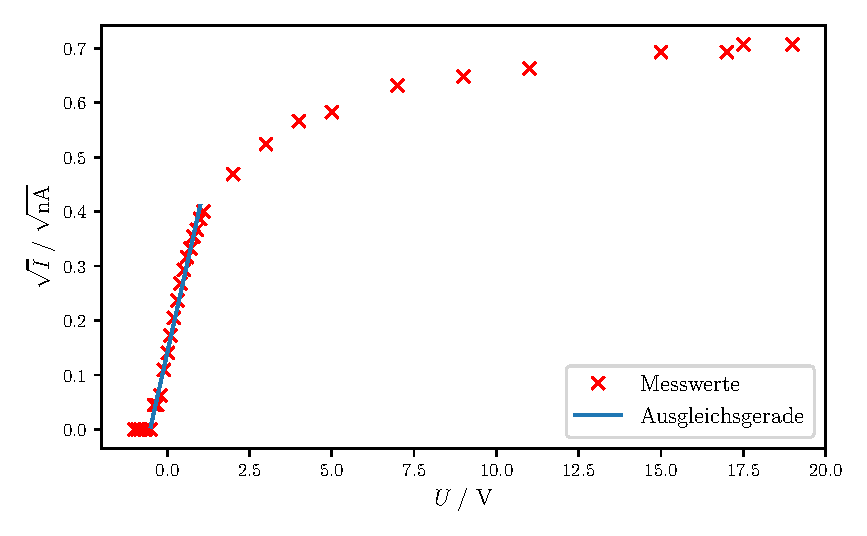
\includegraphics{gelb.pdf}
    \caption{Grafik zur Bestimmung der Gegenspannung für gelbeses Licht $ \lambda = 579,1\,\text{nm}$.}
    \label{fig:gelb}
  \end{figure}
  \noindent
  \begin{table}[H]
    \centering
    \caption{Die Messdaten von grünes Licht $\lambda = 579,1 \,\text{nm}$ }
    \label{tab:grün}
    \begin{tabular}{| c | c |c||c|c|c| }
    \toprule
    $U/\mathrm{V}$ &$I/\mathrm{nA}$  &  $\sqrt{I}/\sqrt{\mathrm{nA}}$&$U/\mathrm{V}$ & $I/\mathrm{A} $& $\sqrt{I}/\sqrt{\mathrm{nA}}$  \\
    \midrule
    
    -0,60 & 	0,000	& 0,000 &	-0,05	&  0,165 &	0,406\\
    -0,50 & 	0,002	& 0,045 &	 0,00	&  0,200 &	0,447\\
    -0,45 & 	0,004	& 0,063 &	 0,10	&  0,275 &	0,524\\
    -0,40 & 	0,008	& 0,089 &	 0,20	&  0,340 &	0,583\\
    -0,35 & 	0,014	& 0,118 &	 0,30	&  0,420 &	0,648\\
    -0,30 & 	0,026	& 0,161 &	 0,40	&  0,480 &	0,693\\
    -0,25 & 	0,044	& 0,210 &	 0,50	&  0,540 &	0,735\\
    -0,20 & 	0,066	& 0,257 &	 0,75	&  0,660 &	0,812\\
    -0,15 & 	0,086	& 0,293 &	 1,00	&  0,780 &	0,883\\
    -0,10 & 	0,130	& 0,361 &		&&\\	
    

      \bottomrule
      \end{tabular}
    \end{table}

  \begin{figure}[H]
    \centering
    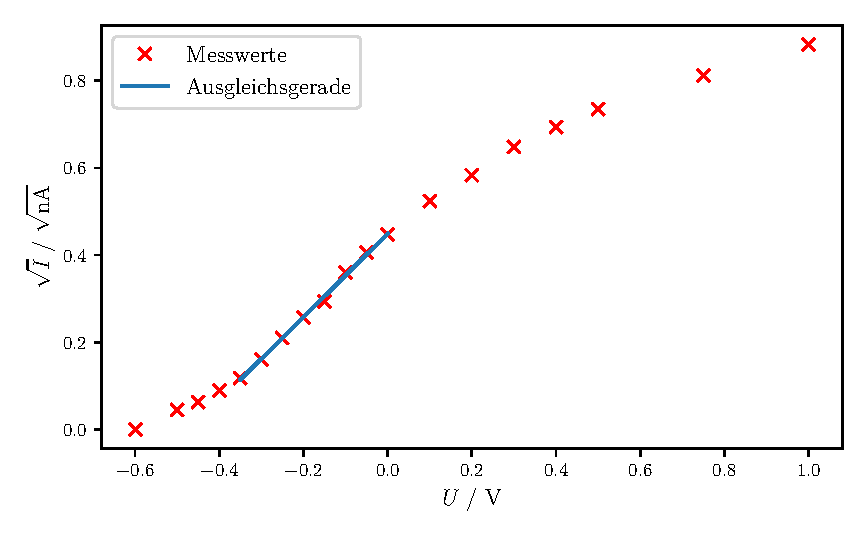
\includegraphics{grün.pdf}
    \caption{Grafik zur Bestimmung der Gegenspannung für grünes Licht $ \lambda = 546\,\text{nm}$.}
    \label{fig:grün}
  \end{figure}
  \noindent
  \begin{table}[H]
    \centering
    \caption{Die Messdaten von blaugrünes Licht $\lambda = 491,6\,\text{nm}$ }
    \label{tab:blaugrün}
    \begin{tabular}{| c | c |c||c|c|c| }
    \toprule
    $U/\mathrm{V}$ &$I/\mathrm{nA}$  &  $\sqrt{I}/\sqrt{\mathrm{nA}}$&$U/\mathrm{V}$ & $I/\mathrm{A} $& $\sqrt{I}/\sqrt{\mathrm{nA}}$  \\
    \midrule
    
    -1,06	& 0,000	& 0,000& 	-0,20	& 0,008	& 0,089 \\
    -1,00	& 0,000	& 0,000& 	-0,15	& 0,008	& 0,089 \\
    -0,95	& 0,000	& 0,000& 	-0,10	& 0,010	& 0,100 \\
    -0,90	& 0,000	& 0,000& 	-0,05	& 0,011	& 0,105 \\
    -0,85	& 0,000	& 0,000& 	0,00	& 0,012	& 0,110 \\
    -0,70	& 0,001	& 0,032& 	0,10	& 0,014	& 0,118 \\
    -0,65	& 0,001	& 0,032& 	0,20	& 0,016	& 0,126 \\
    -0,60	& 0,002	& 0,045& 	0,30	& 0,020	& 0,141 \\
    -0,55	& 0,002	& 0,045& 	0,40	& 0,022	& 0,148 \\
    -0,50	& 0,002	& 0,045& 	0,50	& 0,024	& 0,155 \\
    -0,45	& 0,003	& 0,055& 	0,60	& 0,026	& 0,161 \\
    -0,40	& 0,004	& 0,063& 	0,70	& 0,028	& 0,167 \\
    -0,35	& 0,004	& 0,063& 	0,80	& 0,032	& 0,179 \\
    -0,30	& 0,005	& 0,071& 	0,90	& 0,034	& 0,184 \\
    -0,25	& 0,006	& 0,077& 	1,00	& 0,036	& 0,190 \\
      \bottomrule
      \end{tabular}
    \end{table}

  \begin{figure}[H]
    \centering
    \includegraphics{blaugrün.pdf}
    \caption{Grafik zur Bestimmung der Gegenspannung für blaugrünes Licht $ \lambda =491,6\, \text{nm}$.}
    \label{fig:blaugrün}
  \end{figure}
  \noindent

  \begin{table}[H]
    \centering
    \caption{Die Messdaten von violetes Licht $\lambda = 435,8 \,\text{nm}$ }
    \label{tab:violet}
    \begin{tabular}{| c | c |c||c|c|c| }
    \toprule
    $U/\mathrm{V}$ &$I/\mathrm{nA}$  &  $\sqrt{I}/\sqrt{\mathrm{nA}}$&$U/\mathrm{V}$ & $I/\mathrm{A} $& $\sqrt{I}/\sqrt{\mathrm{nA}}$  \\
    \midrule
    -1,12	& 0,000 &	0,000	& -0,50	& 0,190	& 0,436 \\
    -1,11	& 0,001 &	0,032	& -0,40	& 0,265	& 0,515 \\
    -1,10	& 0,002 &	0,045	& -0,30	& 0,340	& 0,583 \\
    -1,08	& 0,003 &	0,055	& -0,20	& 0,440	& 0,663 \\
    -1,05	& 0,004 &	0,063	& -0,10	& 0,520	& 0,721 \\
    -1,00	& 0,008 &	0,089	& 0,00	& 0,620	& 0,787 \\
    -0,95	& 0,014 &	0,118	& 0,10	& 0,720	& 0,849 \\
    -0,90	& 0,022 &	0,148	& 0,20	& 0,820	& 0,906 \\
    -0,85	& 0,030 &	0,173	& 0,30	& 0,920	& 0,959 \\
    -0,80	& 0,042 &	0,205	& 0,40	& 1,000	& 1,000 \\
    -0,75	& 0,056 &	0,237	& 0,60	& 1,200	& 1,095 \\
    -0,70	& 0,076 &	0,276	& 0,80	& 1,400	& 1,183 \\
    -0,60	& 0,125 &	0,354	& 1,00	& 1,550	& 1,245 \\
    
    

       \bottomrule
      \end{tabular}
    \end{table}

  \begin{figure}[H]
    \centering
    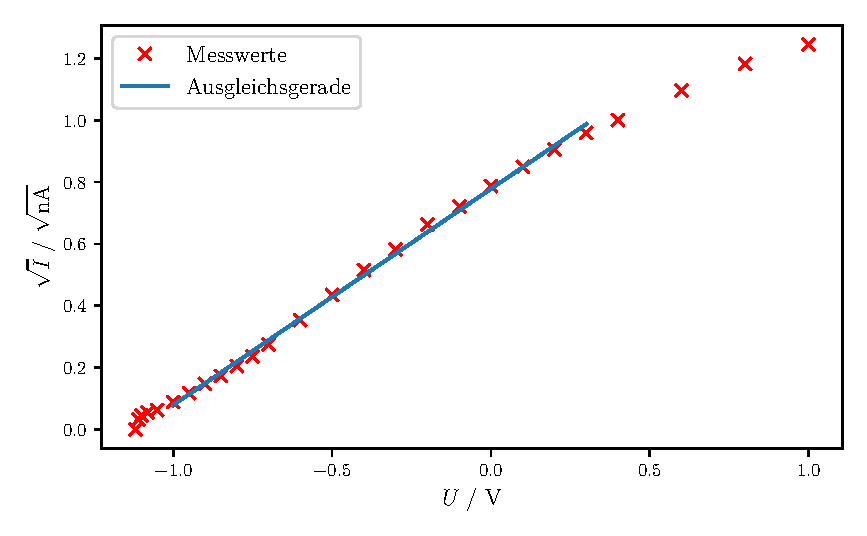
\includegraphics{violet.pdf}
    \caption{Grafik zur Bestimmung der Gegenspannung für violetes Licht $ \lambda = 435,8\,\text{nm}$.}
    \label{fig:violetes}
  \end{figure}
  \noindent
Die Parameter  der Ausgleichungsgeraden und der Wert von der Gegenspannung sind  in Tabelle \ref{tab:Gegenspannung} aufgelistet.
\begin{table}[H]
  \centering
  \caption{Die Gegenspannungen verschiedener monochromatischen Lichtern.}
  \label{tab:Gegenspannung}
  \begin{tabular}{| c |c|c|  c |}
  \toprule
   $\lambda/\mathrm{nm}$ & $a/\mathrm{\dfrac{\sqrt{nA}}{V}}$  &  $b/\mathrm{\sqrt{nA}}$& $U_g/\mathrm{V}$  \\
   \midrule
   640& $0,320 \pm 0,007 $&$0,074\pm 0,001$&      $  -0,231 \pm 0,006 $\\
   579,1& $0,270 \pm 0,008$& $0,141\pm 0,004$&    $  -0,522 \pm 0,021 $\\
   546&$0,956 \pm 0,020 $ & $0,449 \pm 0,004$ &   $ -0,470 \pm  0,011 $\\
   491,6&$0,116 \pm 0,004 $ & $0,109 \pm 0,002$ & $-0,940 \pm   0,037 $\\
   435,8& $0,699 \pm 0,004 $ & $0,778 \pm 0,002$& $-1,113\pm    0,007 $\\

  \bottomrule
  \end{tabular}
\end{table}


\subsection{Bestimmung des Verhältnisses $h/e_0$ und der Austrittsarbeit $A_k$}
Aus der Gleichung (5) folgt die Zusammenhang
\begin{equation}
  U_g= -\frac{h}{e_0}\cdot \nu -\frac{A_k}{e_0}.\\
\end{equation}
Dabei wird die Lichtfrequenz durch Gleichung (2) bestimmt.
Die berechneten Werten zur Bestimmung des Verhältnisses $h/e_0$ und der Austrittsarbeit $A_k$ sind in Tabelle \ref{tab:Austritt} aufgelistet.
\begin{table}[H]
  \centering
  \caption{Die Messdaten zur Bestimmung des Verhältnisses $h/e_0$ und der Austrittsarbeit $A_k$.}
  \label{tab:Austritt}
  \begin{tabular}{| c | c |c|}
  \toprule
   $\lambda/\mathrm{nm}$ & $\nu/\mathrm{ 10^{14}\,Hz}$& $U_g/\mathrm{V}$  \\
  \midrule
  640&   4,688   & $  -0,231 \pm 0,006 $  \\
  579,1& 5,180 &   $  -0,522 \pm 0,021 $\\
  546 &  5,495  &  $ -0,470 \pm  0,011 $ \\
  491,6& 6,103  &  $-0,940 \pm   0,037 $  \\
  435,8& 6,884  &  $-1,113\pm    0,007 $\\
  \bottomrule
  \end{tabular}
\end{table}
\noindent
Die Lichtfrequenz wird gegen die jeweilige Gegenspannung aufgetragen (siehe Grafik \ref{fig:gegenspannung}).
\begin{figure}[H]
  \centering
  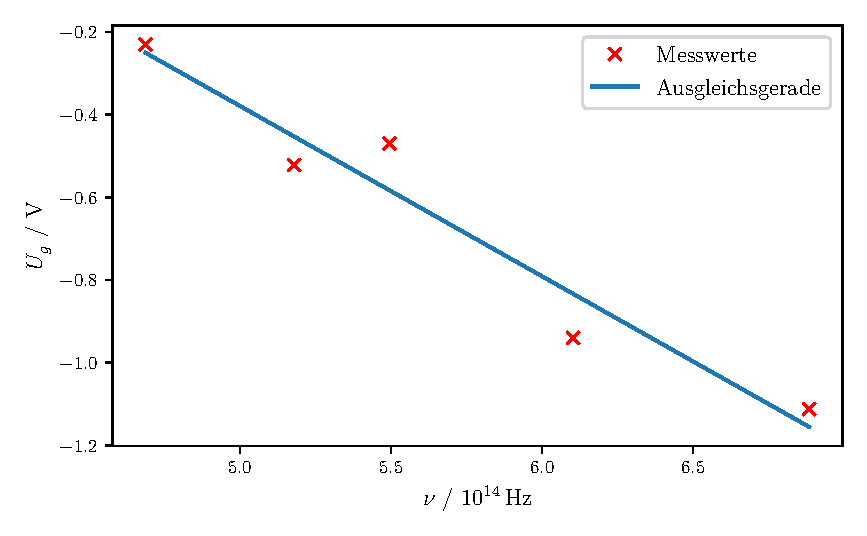
\includegraphics{gegenspannung.pdf}
  \caption{Grafik zur Bestimmung des Verhältnisses $h/e_0$ und der Austrittsarbeit $A_k$.}
  \label{fig:gegenspannung}
\end{figure}
\noindent
Die Ausgleichsgerade besitz die Form:
\begin{equation}
 U_g=a\cdot \nu +b 
\end{equation}
mit \begin{align*}
  a &=-\frac{h}{e_0},\\
  b&=-\frac{A_k}{e_0}.\\
\end{align*}
Die Parameter ergeben sich zu
\begin{align*}
  a &=(-0,412\pm 0,060)\cdot\mathrm{10^{-14}\,\frac{Js}{C}} \\
  b &=(-1,681 \pm 0,342 )\,\mathrm{V} .\\
 \end{align*}
 \noindent
 Somit sind
 \begin{align*}
  \frac{h}{e_0} &=(0,412\pm 0,060)\cdot \mathrm{10^{-14}\,\frac{Js}{C}} \\
  A_k &=( 1,681 \pm 0,342 )\,\mathrm{eV} .\\
 \end{align*}
 \noindent
 Das Verhältnis $h/e_0$ lässt sich theoretisch auch über eine Division des Plank'schen Wirkungsquantums \cite{2} durch die Elementarladung \cite{3} bestimmen, daraus folgt:
\begin{eqnarray}
\nonumber
\frac{6,62607015 \cdot 10^{-34} \, \text{Js}}{1,6021765\cdot 10^{-19} \, \text{C}} =  4,136 \cdot 10^{-15}   \, \mathrm{\frac{Js}{C}}.
\end{eqnarray}
Das Verhältnis $h/e_0$  werden  mit dem theoretischen Wert verglichen, somit ergeben sich nach  
\begin{equation}
  \nonumber
  \text{Abweichung} = \Big\vert\frac{\text{Berechnete Werte}-\text{Literaturwerte}}{\text{Literaturwerte}}\Big\vert \cdot 100 \%
\end{equation}
die Abweichungen von  $ 0,387 \, \% $,
 diese mag an der geringen Anzahl von Messwerten im linearen Bereich liegen. 
 Bedingt durch die Fermi-Verteilung wird zwar eine etwas höhere Gegenspannung gemessen, 
 dies bewirkt allerdings lediglich eine Verschiebung der Geraden, ihre Steigung und somit das Verhältnis 
 sind hiervon natürlich nicht beeinflusst.\\
  Bedingt durch diesen Effekt verschiebt sich allerdings
  die Austrittsarbeit ein wenig, doch ist dieser Effekt so klein, das er vernachlässigt werden 
  kann gegen den Fehler der Austrittsarbeit. Hier lässt sich hier kein theoriewert  für die Austrittsarbeit bestimmen,
  da nicht bekannt ist, aus welchem Material die Kathode ist.


 \subsection{Deutung der Kurve }
 \begin{figure}[H]
  \centering
  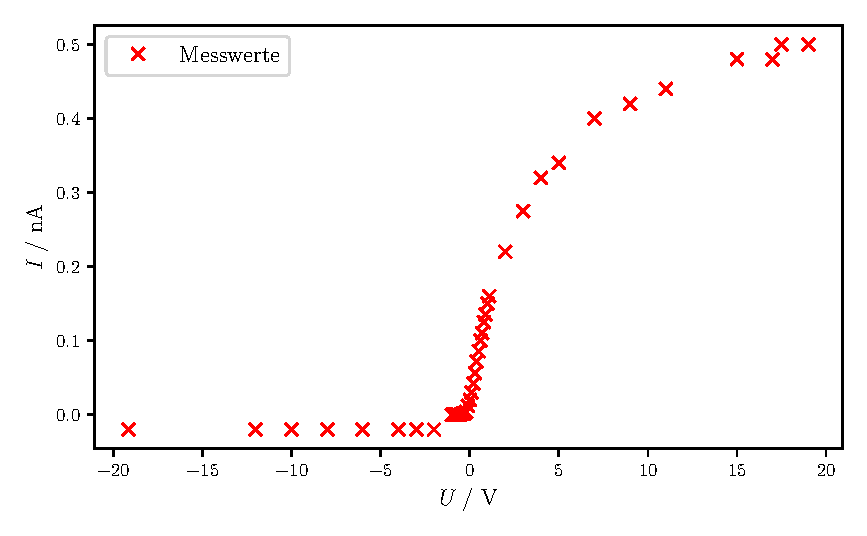
\includegraphics{deutung.pdf}
  \caption{Strom I gegen Spannung U für  $\lambda = 579,1  \, \text{nm}$.}
  \label{fig:deutung}
\end{figure}
\noindent
 Der in Abbildung \ref{fig:deutung} dargestellten Kurvenverlauf wird mit folgenden betrachtet. \\
 Die Kurve erreicht bei hohen beschleunigende Spannungen einen  Sättigungswert  i.h.v $0,5\, \text{V}$, die bedingt dadurch ist, 
dass nur eine endliche Anzahl von Elektronen auf der Kathode vorhanden ist.
Der Photostrom ist proportional zur Lichtintensität und nicht zur Spannung, 
und kann somit selbst bei sehr hohen Spannungen einen Grenzwert nicht überschreiten. 
Die Sättigung ist erreicht, wenn alle Elektronen der Kathode die Anode erreichen können.
Dieser Sättigungswert wird allerdings nur asymptotisch erreicht,
da auch wenn die Elektronen sich geradlinig bewegen, sie einer gewissen Streuung unterliegen. 
Dadurch erreichen nicht alle die gegenüberlegende Anode. 
Zur verbesserung dieses Aufbaus, müsste die Lichtquelle ins Innere einer geschlossenen, kugelförmigen Anode 
gebracht werden und dort die ebenfalls im Innern befindliche Kathode bestrahlen. 
Somit würden zwangsläufig alle Elektronen auch die Anode erreichen können, unabhängig von ihrer Streuung. \\
Weiter beginnt der Photostrom schon vor dem Erreichen der Gegenspannung zu sinken.
 Dies wird mittels der Fermi-Dirac-Statistik erklärt, da nicht alle Elektronen die das Licht auslöst,
  die gleiche Energie haben. \\
Dem Photostrom entgegengerichtet tritt, wie festgestellt wurde ein weiterer Strom auf,
 da sich auch an der Anode ein lichtelektrischer Effekt ereignet.
 Bedingt durch die deutlich kleinere Oberfläche der Anode fällt allerdings dieser Strom viel geringer aus. 
 Theoretisch müsste gelten, dass die Austrittsarbeit der Anode einen deutlich grö"seren Betrag besitzen müsste als die der Kathode,
  da sie zweckmä"sig aus einem Material mit grö"serer Bindungsenergie gefertigt ist. 
  Allerdings besteht die Kathode aus einem Material, das bereits bei $T= 20° \text{C}$ merklich verdampfen kann.
Bedingt durch das Vakuum können sich nun diese verdampften Teilchen an der Anode ablagern und bilden so eine neue Oberfläche mit geringerer Austrittsarbeit, 
die wahrscheinlich mit der Zeit sich dem Wert der Kathode nähert.
 Schon jetzt ist eine gro"se Nähe beider Werte der Grenzspannung leicht zu sehen, 
 auf grund des zu geringen Auflösungsvermögens des Amperemeters lässt sich allerdings in diesem Bereich nichts
  näheres darüber feststellen. Die relativ keinen Sättigungsbeträge lassen sich erklären durch die relative grö"se der Kathode zur Anode,
   wodurch der negative Photostrom schon bei kleinen Lichtintensitäten die Kathode erreichen können, 
   ohne eine grö"se Spannung zu benötigen. 












